
{\underline {\bf Во второй главе}} проведен анализ АКМ.
Множеством характеристик пользователей АКМ является
множество объектов $I$, вес характеристики --- это значение $\rho(u, i)$.
Если мощность множества $P_0$ мала, то правила вывода АКМ
не могут быть применены.
С малой мощностью данных связаны такие известные проблемы АКМ, как
разреженность матрицы (data sparsity) и холодный старт.

Реальные исходные данные обладают свойствами динамики и
неоднородности.
Свойство динамики заключается в том, что множество исходных данных
меняется во времени, так как меняются предпочтения пользователей, и
мощность множеств $U$, $I$ растет.
Пусть $u_a \ru u \text{ для } P_0$, но в силу динамики возможна ситуация, когда
$\rhu(u_a, u) > \varepsilon_p \text{ для } P_{\bot}$. Тогда
утверждение СОМ (\ref{srs-assert}) и, следовательно, правило $\Pi_C$
(\ref{srs-pi}) ложны в общем случае для любых исходных данных.

Свойство неоднородности заключается в том, что пользователи предпочитают
различные, не обязательно близкие по характеристикам, объекты, то есть
предпочтения пользователей не однородны:
$\forall i, j:  (u_a \R i) \wedge (u_a \R j) \not \Rightarrow (i \rt j)$.
Тогда $\forall i, j:  (u_a \R i) \wedge (i \rt k) \not \Rightarrow u_a \R k$,
то есть утверждение ООМ (\ref{ors-assert}) и, следовательно, правило $\Pi_O$
(\ref{ors-pi}) ложны в общем случае для любых исходных данных.

Таким образом, если данные обладают свойством неоднородности или динамики,
то СОМ или ООМ не гарантируют получение качественного решения
в общем случае.

Пусть правила $\Pi_C$ и $\Pi_O$
истинны (то есть выполняются эвристические утверждения). Рассмотрим условия,
которые влияют на качество решения.

В исследовании было определено достаточные условие,
при выполнении которых СОМ и ООМ гарантируют получение качественного
решения задачи $pred$.

Достаточным условием получения качественного решения задачи $pred$
в СОМ является выполнение транзитивности отношения близости на
кластере соседей: $\forall u_1, u_2 \in \mathcal{N}_U: (u_1 \ru u_a) \wedge
(u_2 \ru u_a) \Rightarrow u_1 \ru u_2$.

Достаточным условием получения качественного решения задачи $topN$ в ООМ
является выполнение транзитивности отношения близости на
объединении обучающего, тестового и результирующего множеств:
$(i \rt j) \wedge (i \rt k) \Rightarrow (j \rt k), i, j, k \in I^a_0 \bigcup
I_{topN} \bigcup I_{\bot}, I_{\bot} = \{i_{\bot}, I_{0} = \{i_{0}\}\}$.

Выполнение достаточных условий зависит от того, какая
функция используется в качестве меры близости и какой пороговый
параметр ($\varepsilon_{i}$ или $\varepsilon_p$) этой функции
установлен для выявления выполнения отношения близости.
Пусть $\rhi$ является функцией косинуса угла между контентами, которые
представляются в виде векторов в ООМ, и $\varepsilon_i = 0,49$, тогда
транзитивность отношения $\rt$ не гарантируется; коэффициент корреляции Пирсона,
являющийся традиционной мерой близости СОМ, не обладает свойством
транзитивности. Разработчики РС должны учитывать выполнение достаточных условий
при подборе функции и ее порогового значения, однако не всегда возможно
подобрать эти параметры так, чтобы выполнялись достаточные условия, и РС
удовлетворяла требованиям заказчика. В общем случае АКМ не являются
качественными моделями.

Вычислительную сложность будем характеризовать асимптотической сложностью
алгоритмов решений. Общее и основное действие, которое производится при
решении задач в ООМ и СОМ
--- вычисление меры близости. Поэтому примем данную операцию элементарной
и вычислим асимптотическую сложность алгоритмов относительно этой операции.
Для решения задачи $topN$ строится матрица, элементами которой являются
значения мер близости между объектами, поэтому
асимптотическая сложность равна $O(n^2)$ (алгоритм представлен на Рис. 1).
\begin{figure}[H]
	\caption{Алгоритм решения задачи $topN$}
	\begin{center}
		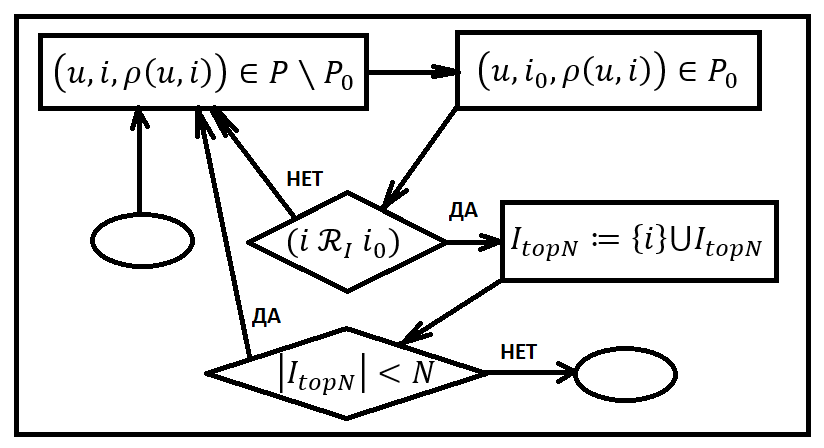
\includegraphics[width=4in,height=2in]{pics/oom_topN.png}
	\end{center}
\end{figure}
Для решения задачи $pred$ необходимо построить множество соседей,
поэтому асимптотическая сложность равна $O(|U|)$ (алгоритм представлен на Рис. 2).
\begin{figure}[H]
	\caption{Алгоритм решения задачи $pred$}
	\begin{center}
		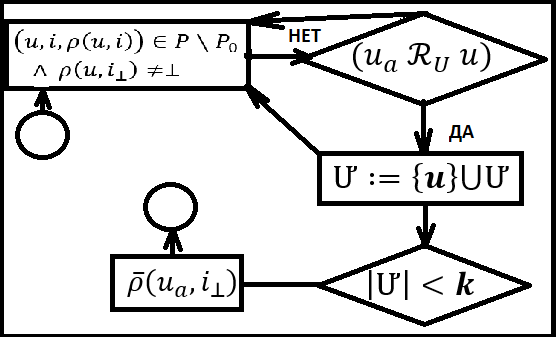
\includegraphics[width=4in,height=2in]{pics/prdn-com.png}
	\end{center}
\end{figure}
Реальные системы, к примеру, Amazon, работают с огромным числом пользователей
(свыше 29 миллионов) и объектов (свыше миллиона), поэтому
асимптотическая сложность алгоритмов решений СОМ и ООМ велика в условиях работы
с подобными массивами данных, которые характерны для реальных данных.
